\chapter{二次函数}

\section{二次函数}
\subsection{函数的奇偶性}

在研究二次函数之前,我们先来研究函数的一个性
质——函数的奇偶性。

我们先来描绘$y=x^2$的图象。

先作出下面的数值表:

\begin{center}
\begin{tabular}{c|ccccccccccc}
    \hline
    $x$   &$\cdots$&   $-2$   &   $-1.6$   &   $-1$   &   $-0.5$   &   $0$   &   $0.5$   &   $1$   &   $1.5$   &   $2$   &   $\cdots$      \\
    \hline
       $y$  &$\cdots$ &   $4$   &   $2.25$   &   $1$   &   $0.25$   &   $0$   &   $0.25$   &   $1$   &   $2.25$   &   $4$   &   $\cdots$\\
       \hline
\end{tabular}
\end{center}

用表里各组对应值作为点的坐标,作出各个点,然后用
平滑的曲线把它们连结起来,就得出$y=x^2$的图象(图5.1),
这个图象叫做抛物线。函数$y=x^2$的图象,以后简称为抛物线
$y=x^2$。

\begin{figure}[htp]
    \centering
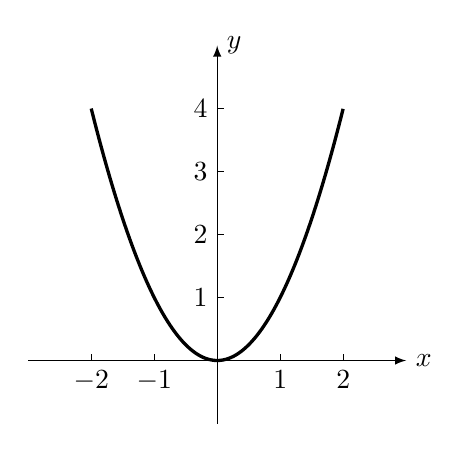
\begin{tikzpicture}[>=latex, scale=.8]
\draw[->](-3,0)--(3,0)node[right]{$x$};
\draw[->](0,-1)--(0,5)node[right]{$y$};
\foreach \x in {-2,-1,1,2}
{
    \draw (\x,0)node[below]{$\x$}--(\x, 0.1);
}
\foreach \x in {1,2,...,4}
{
    \draw (0,\x)node[left]{$\x$}--(.1,\x);
}

\draw[domain=-2:2, samples=100, very thick] plot(\x,{\x*\x});

\end{tikzpicture}
    \caption{}
\end{figure}


从上面表格中可以看到这个函数有一个特点:当自变量
取绝对值相等而符号相反的两个值时(如$x$取1.5和$-1.5$),
它们对应的函数值相等($y$都取2.25),这说明$y$轴垂直平分以
点$(x,f(x))$, $(-x,f(-x))$为端点的线段,换句话说,点
$(x,f(x))$, $(-x,f(x))$是关于$y$轴对称的,因此抛物线$y=x^2$
是关于$y$轴对称的。

我们把具有这种特征
的函数叫做偶函数。$f(x)$
是偶函数的标志是:当自
变量$x$取一对互为相反
数的值时,函数的值不
变,就有$f(x)=f(-x)$。

一般地说,对于函数
$f(x)$, 设$x$和$-x$都属于函
数的定义域,如果
\[f(-x)=f(x)\]
那么函数$f(x)$叫做\textbf{偶函数},偶函数的图象关于$y$轴对称。

我们再来画函数$y=\frac{1}{8}x^3$的图象

先作出下面的数值表:
\begin{center}
\begin{tabular}{c|ccccccccccc}
    \hline
    $x$ &$\cdots$&$-4$&$-3$&$-2$&$-1$&0&1&2&3&4&$\cdots$\\
\hline
$y$ &$\cdots$&$-8$&$-3\frac{3}{8}$&$-1$&$-\frac{1}{8}$&0&$\frac{1}{8}$&1&$3\frac{3}{8}$&8&$\cdots$\\
\hline
\end{tabular}
\end{center}

根据表里这些对应值,作出函数$y=x^3$的图象如图
5.2。这个图象称为立方抛物线。
\begin{figure}[htp]
    \centering
\begin{tikzpicture}[>=latex, scale=.5]
\draw[->](-5,0)--(5,0)node[right]{$x$};
\draw[->](0,-9)--(0,9)node[right]{$y$};
\foreach \x in {1,2,3,4}
{
    \draw (\x,0)node[below]{$\x$}--(\x, 0.1);
}
\foreach \x in {-2,-4}
{
    \draw (\x,0)node[above]{$\x$}--(\x, -0.1);
}
\foreach \x in {-8,-6,...,-2,2,4,...,8}
{
    \draw (0,\x)node[left]{$\x$}--(0.1,\x);
}
\node at (-.5,-.5){$O$};
\draw[domain=-4:4, samples=100, very thick] plot(\x,{\x*\x*\x/8});

\end{tikzpicture}
    \caption{}
\end{figure}

从上面表格中可以看到这个函数也有一个特征:因为,
$\frac{1}{8}(-x)^3=-\frac{1}{8}x^3$, 所以当自变量取两个互为相反数的值时,
对应的函数值也是互为相反数。所以如果点$(x,f(x))$在函
数的图象上,那么必有另一点$(-x,-f(x))$也在函数的图象
上,而原点恰是以$(x,f(x))$, $(-x,-f(x))$为端点的线段
的中点,换句话说,点$(x,f(x))$, $(-x,-f(x))$是关于原
点对称的。因此立方抛物线
$y=\frac{1}{8}x^3$是关于原点对称的,我
们把具有这种特征的函数叫做
奇函数,$f(x)$是奇函数的标志
是:当自变量$x$取一对互为相
反数的值时,函数的值也是
互为相反数,就是$f(-x)=-f(x)$。

一般地说,对于函数$f(x)$, 设$x$与$-x$都属于函数的定义
域,如果$$f(-x)=-f(x)$$ 那么函数$f(x)$叫做\textbf{奇函数}。奇函数的图象关于原点对称。

考虑一个函数是偶函数、奇函数,或者既不是偶函数又
不是奇函数,叫做研究函数的奇偶性,对于一个奇函数或者
偶函数,要了解它的性质和图象,只要了解当自变量取正
值时的性质和图象就可以了。例如,要作函数$y=\frac{1}{8}x^3$的图
象,因为它是奇函数,所以只要作出自变量取正值时的函数
图象,就可以利用奇函数的图象必定关于原点对称这一特点,
作出自变量取负值时的图象。















